%\subsubsection*{Tensor Polarization}
When a  spin 1 system such as the deuteron is subjected to a magnetic field along the z-axis, the
Zeeman interaction gives rise to three magnetic sublevels $I_z = +1,0,-1$ with
population fractions $p_+,p_-, p_0$, respectively.
%\footnote{i.e. $p_+ + p_- +p_0=1$.}.
These populations are described by
both a vector  polarization,
%
\begin{eqnarray}
\nonumber
P_z &=&\langle I_z/I\rangle \\
    &=&(p_+ - p_0) + (p_0-p_+) = p_+ - p_-
\end{eqnarray}
and a tensor polarization~\cite{Meyer:1985dta}:
\begin{eqnarray}
\nonumber
P_{zz} &=& \langle 3 I_z^2 - I(I+1)\rangle/I^2   \\
&=&(p_+ - p_0) - (p_0-p_-) = 1 - 3 p_0
\end{eqnarray}
%
which are subject to the overall normalization $p_+ + p_- + p_0 = 1$.

Fig.~\ref{fig:deuteron} graphically demonstrates the dependence of the two nucleon distribution on the spin projection.  If the two nucleons are in a relative $m=0$ state, the surface of constant density is toroidal, while if they are in the $m=\pm 1$ state, the surface has a dumbbell shape.

\begin{figure}
\centering
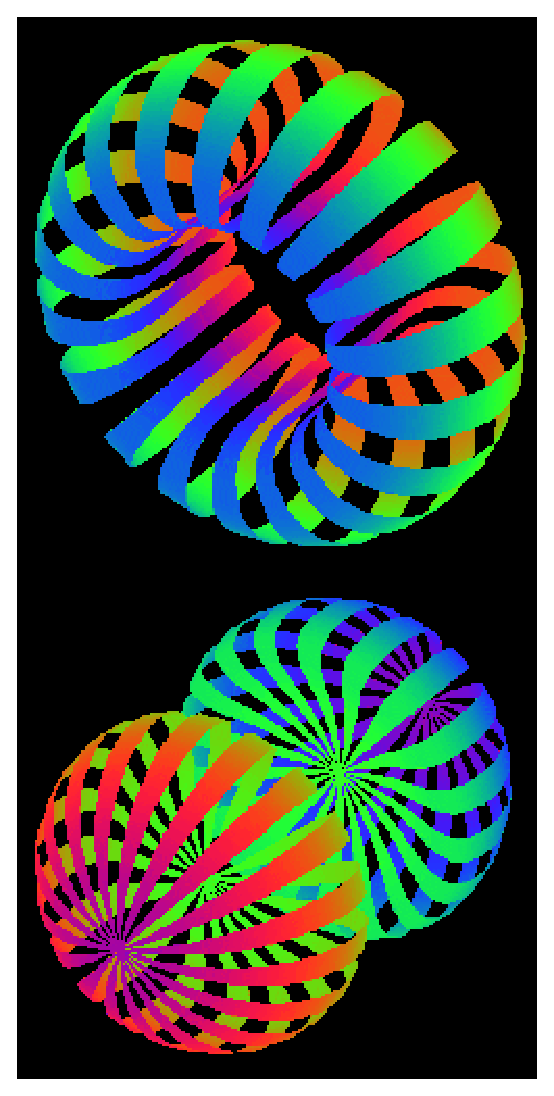
\includegraphics[width=0.3\textwidth,angle=90]{figs/pic-v10-st16-1.eps}
\caption{\label{fig:deuteron}
Nucleon densities of the deuteron in its two spin projections, $I_z=0$ and $I_z=\pm 1$, respectively.
{\it Reproduced from~\cite{Carlson:1997qn,Forest:1996kp}}.
}
\end{figure}

In the case of deuteron spins in thermal equilibrium with the solid lattice, and neglecting the small quadrupole interaction~\cite{Meyer:1985dta}, the tensor polarization is related to  the vector polarization via:
\begin{eqnarray}
\label{TENSORVECTOR}
P_{zz}= 2 - \sqrt{4-3 P_z^2}
\end{eqnarray}
The maximum absolute value of $P_{zz}=-2$  occurs only for vanishing populations in the $m=\pm 1$ states.
If, on the other hand, only the $m=1$ or $m=-1$ state are occupied, the vector polarization reaches its maximum value of $+1$, and $P_{zz}=+1$.  
